
\documentclass[a4paper, 10pt]{IEEEconf}  

\usepackage{geometry}
\geometry{a4paper, margin=1in}
  
  
\usepackage{subcaption}  
\usepackage[export]{adjustbox}    
\usepackage{verbatim}
\usepackage{graphicx}
\usepackage{pdfpages}
\usepackage{cite}
\usepackage{listings}
\usepackage{float}
\usepackage{url}
\usepackage{hyperref}
\usepackage{fancyhdr}
\usepackage{multicol}

\lstset{
	tabsize=2,
	breaklines=true
}

\setlength{\parskip}{1em}
\onecolumn

\title{\LARGE \bf Assignment 2: Engineering Documentation\\Industrial Systems Design and Integration 282 772}
\author{Marc Alexander Sferrazza \\ 12164165
\thanks{This work was not supported by any organization}
\thanks{Faculty of Mechatronics Engineering, Massey University, Albany, Auckland, New Zealand
        {\tt\small Progress of project: https://github.com/alex1v1a/Industrial-Systems-Design-and-Integration} } }

\begin{document}

\maketitle
%\begin{figure}[h]
%\begin{subfigure}{0.5\textwidth}
%\includegraphics[width=1.5\textwidth, left]{images/ROS} 
%%\caption{ROS}
%\label{fig:ROS}
%\end{subfigure}
%\begin{subfigure}{0.5\textwidth}
%\includegraphics[width=0.3\textwidth, right]{images/gazebo}
%%\caption{Gazebo} 
%\label{fig:Gazebo}
%\end{subfigure}
%%\caption{Caption for this figure with two images}
%%\label{fig:image2}
%\end{figure}
%\begin{figure}[H]
%  \begin{center}
%  
\includegraphics[width=110mm]{images/tf}
%  \label{fig:kinetic}
%  \end{center}
%\end{figure}
\thispagestyle{empty}
\pagestyle{plain}


%%%%%%%%%%%%%%%%%%%%%%%%%%%%%%%%%%%%%%%%%%%%%%%%%%%%%%%%%%%%%%%%%%%%%%%%%%%%%%%%

\begin{abstract}

This documentation contains a brief summary of key points regarding this assessment is to explore methods of producing quality engineering documentation. Please explore the directory tree and view the readme files for explanation and overview of documents within.

\end{abstract}


\clearpage
\thispagestyle{empty}
\tableofcontents
\begingroup
\let\clearpage\relax
\listoffigures
%\listoftables
\endgroup
%\thispagestyle{empty}
\clearpage
\twocolumn

%%%%%%%%%%%%%%%%%%%%%%%%%%%%%%%%%%%%%%%%%%%%%%%%%%%%%%%%%%%%%%%%%%%%%%%%%%%%%%%%
%%%%%%%%%%%%%%%%%%%%%%%%%%%%%%%%%%%%%%%%%%%%%%%%%%%%%%%%%%%%%%%%%%%%%%%%%%%%%%%%
\clearpage
\setcounter{page}{1}
%\thispagestyle{empty}
\onecolumn

\section{INTRODUCTION}
This document contains a summary of features for this project; these are quick highlights relating to the assessment specification. For full information on any given topic please use the folder navigation to the correct directory where the original images and files used in this document can be found.

%%%%%%%%%%%%%%%%%%%%%%%%%%%%%%%%%%%%%%%%%%%%%%%%%%%%%%%%%%%%%%%%%%%%%%%%%%%%%%%%
%%%%%%%%%%%%%%%%%%%%%%%%%%%%%%%%%%%%%%%%%%%%%%%%%%%%%%%%%%%%%%%%%%%%%%%%%%%%%%%%

\section{PCB DESIGN (Electronic Subsystem Documentation)}
This PCB was design with Altium, for more information and a Bill of Materials CSV please view the folder PCB DESIGN (Electronic Subsystem Documentation)/CHARGER/PCB Design/Altium

%%%%%%%%%%%%%%%%%%%%%%%%%%%%%%%%%%%%%%%%%%%%%%%%%%%%%%%%%%%%%%%%%%%%%%%%%%%%%%%%

\subsection{PCB Layout}
\begin{figure}[H]
  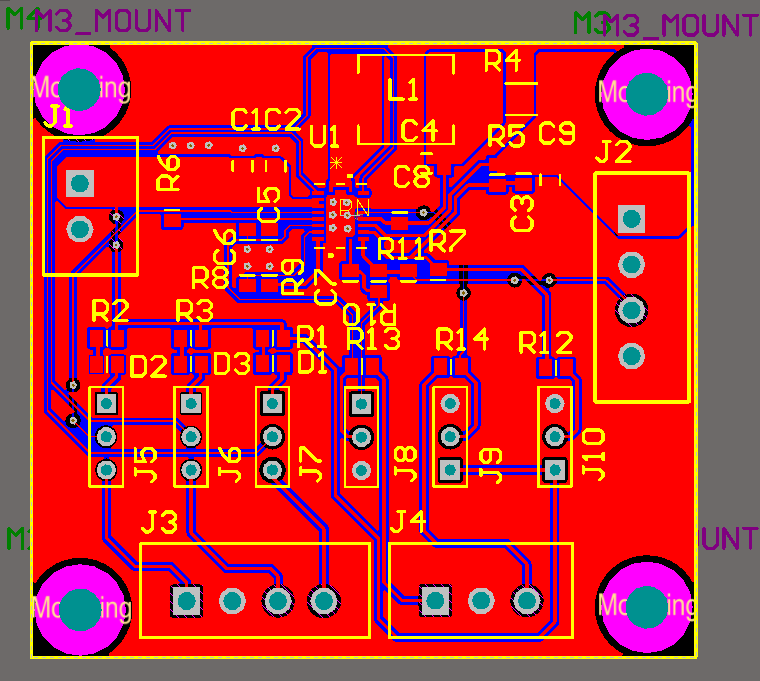
\includegraphics[width=\linewidth, center]{images/PCBLayout}
  \caption{PCB Layout}
  \label{fig:PCB Layout}
\end{figure}

%%%%%%%%%%%%%%%%%%%%%%%%%%%%%%%%%%%%%%%%%%%%%%%%%%%%%%%%%%%%%%%%%%%%%%%%%%%%%%%%

\subsection{Schematic Capture}
\begin{figure}[H]
  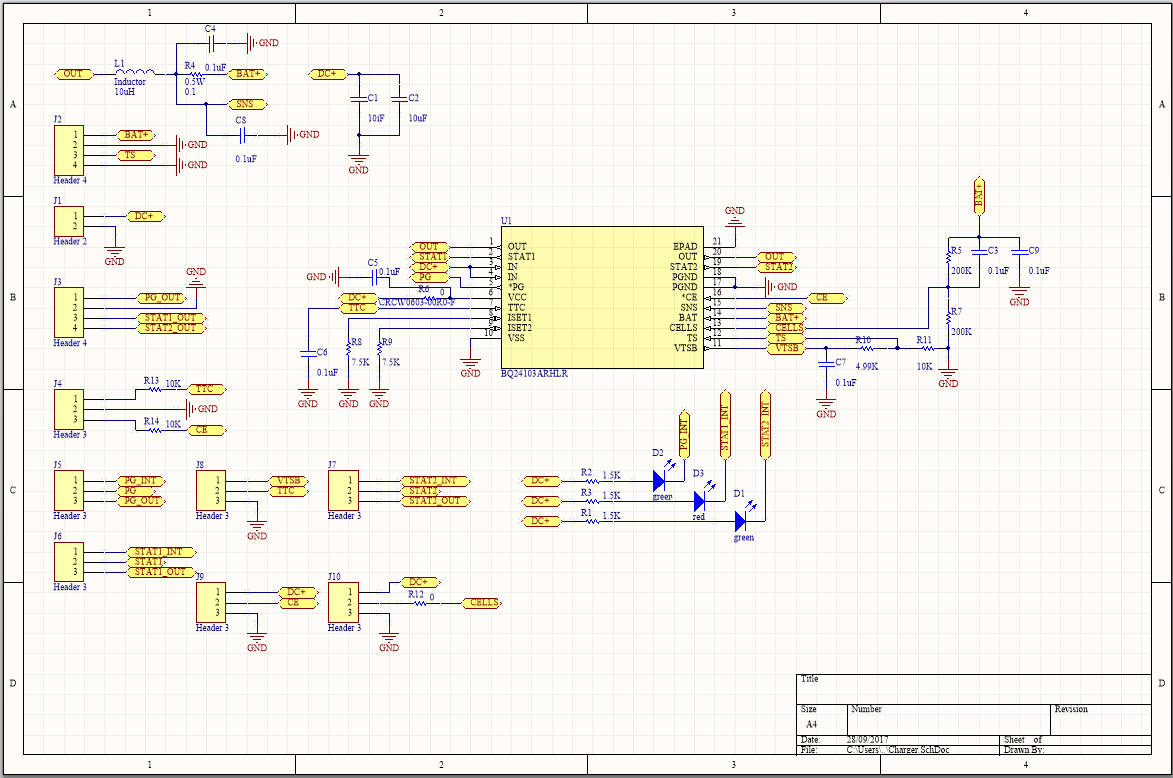
\includegraphics[width=\linewidth, center]{images/SchematicCapture}
  \caption{Schematic Capture}
  \label{fig:Schematic Capture}
\end{figure}

%%%%%%%%%%%%%%%%%%%%%%%%%%%%%%%%%%%%%%%%%%%%%%%%%%%%%%%%%%%%%%%%%%%%%%%%%%%%%%%%
%%%%%%%%%%%%%%%%%%%%%%%%%%%%%%%%%%%%%%%%%%%%%%%%%%%%%%%%%%%%%%%%%%%%%%%%%%%%%%%%
\clearpage
\section{PROJECT BUILD DESIGN (Mechanical Subsystem Documentation)}
These computer aided mechanical designs are made with a combination of Solid works and Adobe illustrator. The entire workspace has been included for clarity in workspace and design including PCB and code. Please view the folder PROJECT BUILD DESIGN (Mechanical Subsystem Documentation)

%%%%%%%%%%%%%%%%%%%%%%%%%%%%%%%%%%%%%%%%%%%%%%%%%%%%%%%%%%%%%%%%%%%%%%%%%%%%%%%%

\subsection{System Architecture Diagram}
This figure shows the systems architecture and how the parts are linked with one another
\begin{figure}[H]
  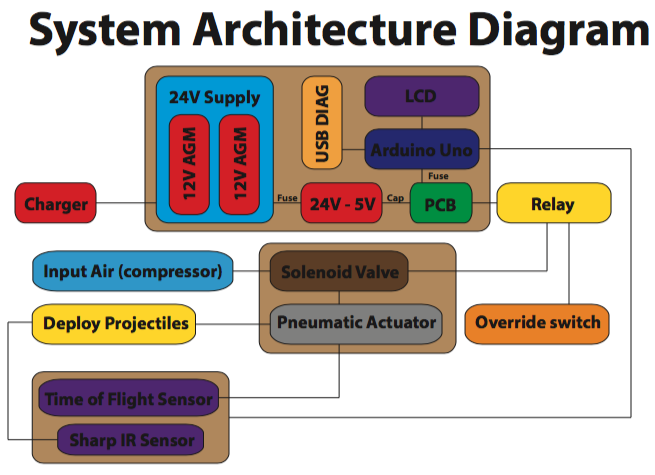
\includegraphics[width=\linewidth, center]{images/SAD}
  \caption{System Architecture Diagram}
  \label{fig:System Architecture Diagram}
\end{figure}

%%%%%%%%%%%%%%%%%%%%%%%%%%%%%%%%%%%%%%%%%%%%%%%%%%%%%%%%%%%%%%%%%%%%%%%%%%%%%%%%
\clearpage
\subsection{Solidworks}
The Following was made with Solidworks 2016, converted from Adobe illustrator. Please ensure to open the CAD files versions 2016 or above is used.
\begin{figure}[H]
  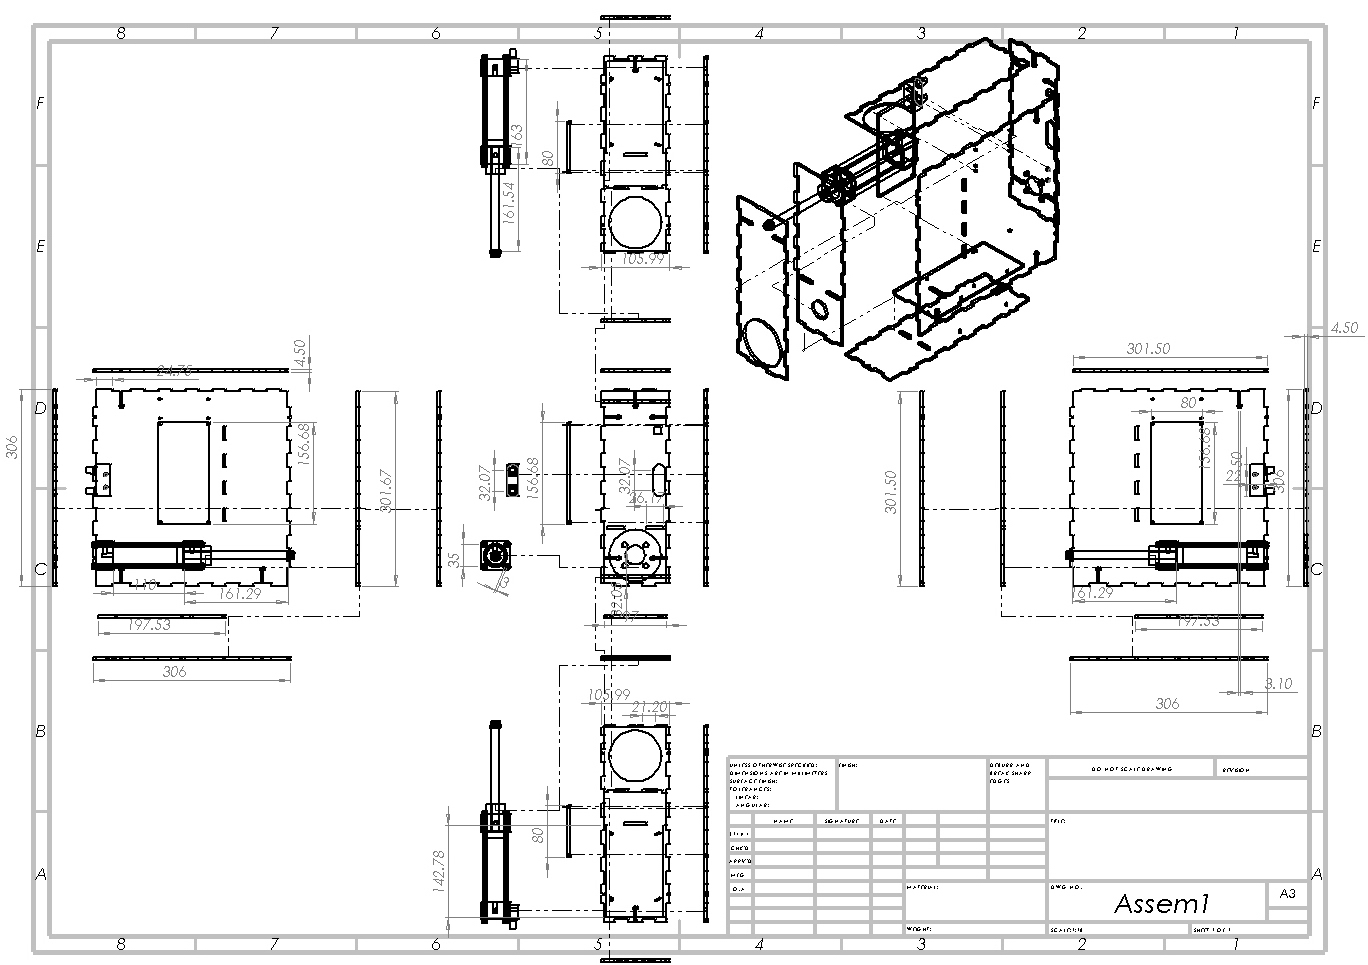
\includegraphics[width=\linewidth, center]{images/Assembly.JPG}
  \caption{Solidworks CAD Assembly Drawing}
  \label{fig:Solidworks CAD Assembly Drawing}
\end{figure}

%%%%%%%%%%%%%%%%%%%%%%%%%%%%%%%%%%%%%%%%%%%%%%%%%%%%%%%%%%%%%%%%%%%%%%%%%%%%%%%%
\clearpage
\subsection{Adobe illustrator - Laser Cut}
Below are the original laser cut files for the project. These files are ready to be directly laser cut and are raster ready.
\begin{figure}[H]
  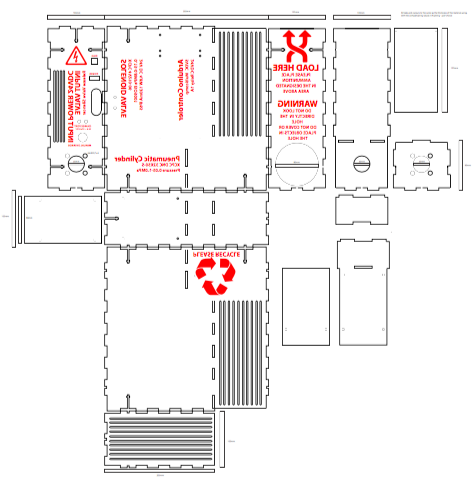
\includegraphics[width=\linewidth, center]{images/QuickView.png}
  \caption{Adobe illustrator - Laser Cut ready for flat pack fold up view}
  \label{fig:Adobe illustrator - Laser Cut ready for flat pack fold up view}
\end{figure}

%%%%%%%%%%%%%%%%%%%%%%%%%%%%%%%%%%%%%%%%%%%%%%%%%%%%%%%%%%%%%%%%%%%%%%%%%%%%%%%%
%%%%%%%%%%%%%%%%%%%%%%%%%%%%%%%%%%%%%%%%%%%%%%%%%%%%%%%%%%%%%%%%%%%%%%%%%%%%%%%%
\clearpage
\section{PROGRAMMING (Soft/Firmware Subsystem Documentation)}
This code selection was made in OpenCV was design with Visual Studio and from source on Mac, for more information and a installation method etc please view the folder 

%%%%%%%%%%%%%%%%%%%%%%%%%%%%%%%%%%%%%%%%%%%%%%%%%%%%%%%%%%%%%%%%%%%%%%%%%%%%%%%%

\subsection{Algorithm Architecture flow diagram}
This can be found in the PROGRAMMING (Soft:Firmware Subsystem Documentation)/OpenCV/Assignment 2 folder, please see the readme files for more information.
\begin{figure}[H]
  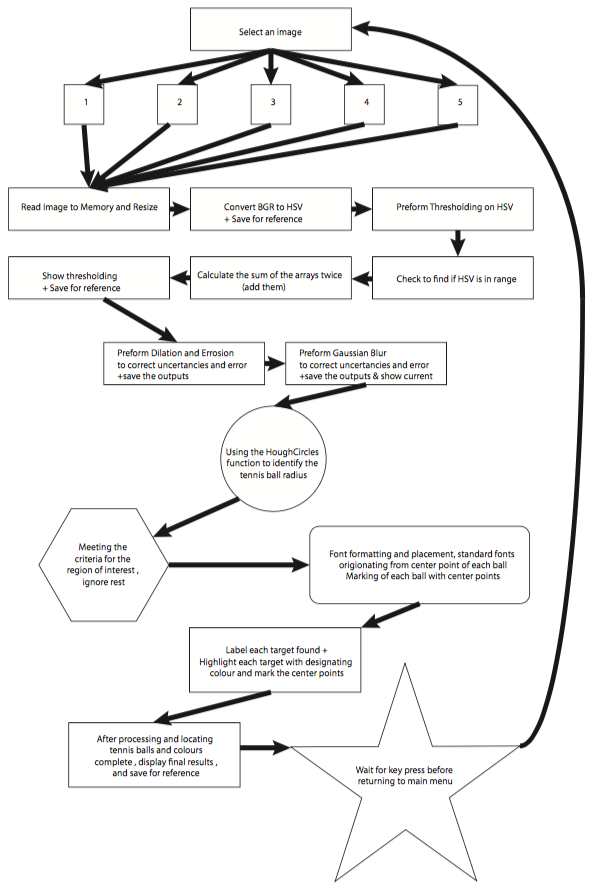
\includegraphics[width=0.7\linewidth, center]{images/AA}
  \caption{Algorithm Architecture flow diagram}
  \label{fig:Algorithm Architecture flow diagram}
\end{figure}
Below is the attached relevant code regarding the flow chart

%%%%%%%%%%%%%%%%%%%%%%%%%%%%%%%%%%%%%%%%%%%%%%%%%%%%%%%%%%%%%%%%%%%%%%%%%%%%%%%%

\clearpage
\onecolumn
\section*{APPENDIX}
\begin{lstlisting}[language = c++]
OPEN CV ASSIGNMENT 2
// Marc Alexander Sferrazza 12164165
// Referenceing from http://docs.opencv.org/2.4/

#include <opencv2\opencv.hpp>
#include <opencv2\core.hpp>
#include <opencv2\imgcodecs.hpp>
#include <opencv2\highgui.hpp>
#include <iostream>
#include <string>
#include <stdio.h>
#include <stdlib.h>
#include <sstream>

using namespace cv;
using namespace std;

void location();

int setpoint;
string name;

int main() {
	cout << "Choose an image to locate the tennis ball: 1, 2, 3, 4, 5...\n\npress esc to quit\n\n-------------------------------------------------------------------------\n" << endl;
	while (1) {
		namedWindow("User Select", CV_WINDOW_AUTOSIZE);
		switch (waitKey(0)) {
		case 27: // Exit prompt "esc"
			return 0;
		case 49: // Image 1 selected
			setpoint = 1;
			name = "1.jpg";
			location();
			break;
		case 50: // Image 2 selected
			setpoint = 2;
			name = "2.jpg";
			location();
			break;
		case 51: // Image 3 selected
			setpoint = 3;
			name = "3.jpg";
			location();
			break;
		case 52: // Image 4 selected
			setpoint = 4;
			name = "4.jpg";
			location();
			break;
		case 53: // Image 5 selected
			setpoint = 5;
			name = "5.jpg";
			location();
			break;
		}
	}
	return 0;
}

void location() {
	Mat image, hsv, thres, dilation, errosion, blur, readyImage, imageFinal;
	
	int yHzLo, yHzHi, yScLo, yScHi, yVrLo, yVrHi;
	int rHzLo, rHzHi, RSLow, rScHi, rVrLo, rVrHi;
	int bHzLo, bHzHi, BSLow, bScHi, bVrLo, bVrHi;
	int roiXmin, roiXmax, roiYmin, roiYmax;
	int r1, r2, r3, b1, b2, b3, y1, y2, y3;
	int hThres, lThres, dis, minRad, maxRad;

	// Naming the saved output files for reference
	ostringstream nameh, namet, named, namee, nameb, namer;
	string namehsv, namethres, namedilation, nameerrosion, nameblur, nameready;
	// Image save locations
	namehsv = "Output/1.HSV Image ";
	namethres = "Output/2.Thresholding Image ";
	namedilation = "Output/3.Dilation Image ";
	nameerrosion = "Output/4.Errosion Image ";
	nameblur = "Output/5.GaussianBlur Image ";
	nameready = "Output/6.Final Result Image ";

	// Read the image to memory and resize
	image = imread(name);
	if (setpoint != 1) {
		resize(image, image, Size(), 0.3, 0.3);
	}
	// Note that the aspect ratio of image 1 is significantly different than the others, these values provide better results
	else if (setpoint = 1) {
		resize(image, image, Size(), 0.5, 0.5);
	}

	// Copy origional image for end results edit
	imageFinal = image;

	// Step 1, Convert BGR to HSV
	cvtColor(image, hsv, COLOR_BGR2HSV);

	// After conversion save for reference
	//imshow("HSV", hsv); //Debugging feature
	nameh << namehsv << setpoint << ".jpg";
	imwrite(nameh.str(), hsv);

	int rval[5][36] = {
		{ 31, 0, 142, 60, 255, 255, 0, 186, 69, 179, 213, 255, 53, 206, 51, 179, 255, 255, 300, 700, 50, 470, 100, 100, 100, 90, 50, 30, 100, 100, 100, 150, 50, 30, 10, 40 },
		{ 153, 148, 128, 179, 227, 255, 90, 121, 0, 114, 255, 255, 22, 63, 148, 89, 198, 255, 260, 700, 170, 470, 110, 100, 100, 100, 130, 50, 140, 180, 110, 150, 50, 30, 10, 40 },
		{ 21, 142, 146, 43, 255, 255, 0, 148, 75, 7, 255, 255, 92, 178, 8, 150, 255, 225, 260, 700, 50, 470, 50, 40, 70, 20, 30,20, 10, 160, 160, 126, 42, 30, 5, 40 },
		{ 18, 194, 57, 35, 255, 255, 0, 190, 69, 6, 255, 255, 107, 176, 45, 112, 255, 255, 260, 700, 50, 470, 60, 65, 67, 34, 85, 88, 100, 100, 100, 82, 34, 30, 10, 40 },
		{ 17, 190, 99, 49, 255, 255, 0, 144, 81, 8, 215, 190, 105, 168, 24, 157, 255, 204, 260, 600, 170, 470, 100, 100, 100, 66, 70, 61, 100, 100, 100, 100, 33, 30, 10, 40 }
	};

	int *propd[36] = {
		&yHzLo, &yScLo, &yVrLo, &yHzHi, &yScHi, &yVrHi,
		&rHzLo, &RSLow, &rVrLo, &rHzHi, &rScHi, &rVrHi,
		&bHzLo, &BSLow, &bVrLo, &bHzHi, &bScHi, &bVrHi,
		&roiXmin, &roiXmax, &roiYmin, &roiYmax,
		&r1, &r2, &r3, &b1, &b2, &b3, &y1, &y2, &y3,
		&hThres, &lThres, &dis, &minRad, &maxRad
	};

	// Set random numbers to the array
	for (int k = 0; k < 36; k++) {
		*propd[k] = rval[setpoint - 1][k];
	}

	// Step 2, Thresholding 
	// Check to find if arrays are in range
	Mat blue, red, yellow;
	inRange(hsv, Scalar(bHzLo, BSLow, bVrLo), Scalar(bHzHi, bScHi, bVrHi), blue);
	inRange(hsv, Scalar(rHzLo, RSLow, rVrLo), Scalar(rHzHi, rScHi, rVrHi), red);
	inRange(hsv, Scalar(yHzLo, yScLo, yVrLo), Scalar(yHzHi, yScHi, yVrHi), yellow);
	
	// Calculate the sum for 2 arrays twice 
	add(blue, red, thres);
	add(thres, yellow, thres);

	// After thresholding save for reference
	//imshow("Thresholding", thres); //Debugging feature
	namet << namethres << setpoint << ".jpg";
	imwrite(namet.str(), thres);

	// Step 3, Dilation and errosion used for multi level channel processing 
	dilate(thres, dilation, getStructuringElement(MORPH_ELLIPSE, Size(11, 11)));
	erode(dilation, errosion, getStructuringElement(MORPH_ELLIPSE, Size(3, 3)));

	// After dilation save for reference
	//imshow("Dilation", dilation); //Debugging feature
	named << namedilation << setpoint << ".jpg";
	imwrite(named.str(), dilation);

	// After errosion save for reference
	//imshow("Errosion", errosion); //Debugging feature
	namee << nameerrosion << setpoint << ".jpg";
	imwrite(namee.str(), errosion);

	// Step 4, Preform Gaussian blur to further bilter image and reduce noise to better detect the raound point for the circles
	GaussianBlur(errosion, blur, Size(7, 7), 2.5, 2.5);

	// After Gaussian blur save for reference
	//imshow("Gaussian Blur", blur); //Debugging feature
	nameb << nameblur << setpoint << ".jpg";
	imwrite(nameb.str(), blur);

	// Assign the filtered image to readyImage for location processing
	readyImage = blur;
	vector<Vec3f> ball;
	Vec3b meanr;

	// Step 5, Using the HoughCircles function to identify the tennis ball radius
	// Originally used the Blob function however this method gave better results
	HoughCircles(readyImage, ball, CV_HOUGH_GRADIENT, 2, dis, hThres, lThres, minRad, maxRad);
	for (size_t k = 0; k < ball.size(); k++) {
		Point center(cvRound(ball[k][0]), cvRound(ball[k][1]));
		// Establish and mark the center points
		int y = center.y, x = center.x;

		// Step 6, Meeting the criteria for the region of interest, ignore rest
		if ((roiXmin < x) && (x < roiXmax) && (roiYmin < y) && (y < roiYmax)) {
			for (int m = x - 5; m < x + 5; m++) {
				for (int n = y - 5; n < y + 5; n++) {
					Vec3b colorr = imageFinal.at<Vec3b>(n, m);
					meanr.val[0] = (colorr.val[0] + meanr.val[0]) / 2;
					meanr.val[1] = (colorr.val[1] + meanr.val[1]) / 2;
					meanr.val[2] = (colorr.val[2] + meanr.val[2]) / 2;
				}
			}

			// Step 7, Font formatting and placement, standard fonts origionating from center point of each ball
			// Marking of each ball with center points
			int font = FONT_HERSHEY_SIMPLEX, thick = 1;
			float scale = 0.5;
			Point org(x, y);
			string colour;

			int radius = int(ball[k][2]);
			if ((meanr.val[0] > b1 && meanr.val[1] < b2 && meanr.val[2] < b3)
				|| (meanr.val[0] == 1 && meanr.val[1] == 252 && meanr.val[2] == 251)) {
				// Label each target found
				colour = "Blue";
				putText(imageFinal, colour, org, font, scale, Scalar(255, 0, 0), thick, 5);
				// Highlight each target with designating colour and mark the center points
				circle(imageFinal, center, radius, Scalar(255, 0, 0), 1, 5, 0);
				circle(imageFinal, center, 3, Scalar(255, 0, 0), 1, 5, 0);
			}
			if (meanr.val[0] < y1 && meanr.val[1] > y2 && meanr.val[2] > y3
				&& (meanr.val[0] != 1 && meanr.val[1] != 252 && meanr.val[2] != 251)) {
				// Label each target found
				colour = "Yellow";
				putText(imageFinal, colour, org, font, scale, Scalar(0, 255, 255), thick, 5);
				// Highlight each target with designating colour and mark the center points
				circle(imageFinal, center, radius, Scalar(0, 255, 255), 1, 5, 0);
				circle(imageFinal, center, 3, Scalar(0, 255, 255), 1, 5, 0);
			}			
			if (meanr.val[0] < r1 && meanr.val[1] < r2 && meanr.val[2] > r3) {
				// Label each target found
				colour = "Red";
				putText(imageFinal, colour, org, font, scale, Scalar(0, 0, 255), thick, 5);
				// Highlight each target with designating colour and mark the center points
				circle(imageFinal, center, radius, Scalar(0, 0, 255), 1, 5, 0);
				circle(imageFinal, center, 3, Scalar(0, 0, 255), 1, 5, 0);
			}
		}
	}
	cout << "Congradulations! Processing complete here are the tennis balls found with their respected colours!\n\npress any key to go back to main menu, or hit esc twice to quit\n\n-------------------------------------------------------------------------\n" << endl;
	// Step 8, After processing and locating tennis balls and colours complete, display final results, and save for reference
	namer << nameready << setpoint << ".jpg";
	imwrite(namer.str(), imageFinal);
	imshow(name, imageFinal); 
	// Wait for key press before returning to main menu
	waitKey(0);
	destroyAllWindows();
}

\end{lstlisting}

\end{document}
